\chapter{Anhang}
\section{Weitere Abbildungen}

\begin{figure}[H]
\begin{center}
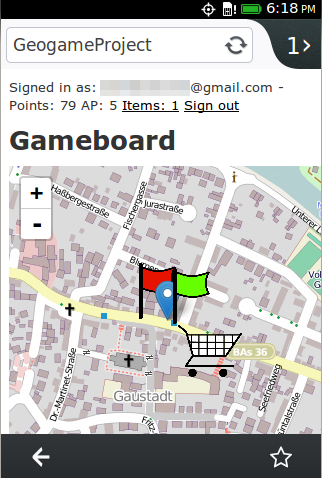
\includegraphics[height=100mm]{images/ch8_firefoxos.png}
\caption{Spielfeld - Smartphone}
\label{img:ch8_firefoxos}
\end{center}
\end{figure}

\begin{figure}[H]
\begin{center}
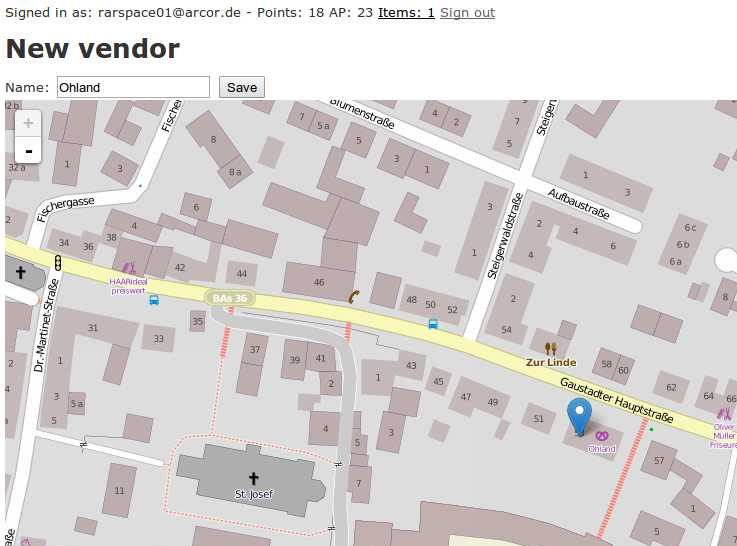
\includegraphics[width=150mm]{images/ch8_vendor_mappick.png}
\caption{Händler Map-Picker}
\label{img:ch8_vendor_mappick}
\end{center}
\end{figure}

\begin{figure}[H]
\begin{center}
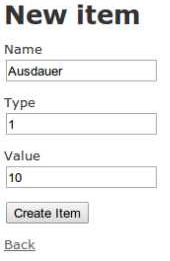
\includegraphics[height=50mm]{images/ch8_item1.png}
\caption{Itempflege - Anlegen}
\label{img:ch8_item1}
\end{center}
\end{figure}

\begin{figure}[H]
\begin{center}
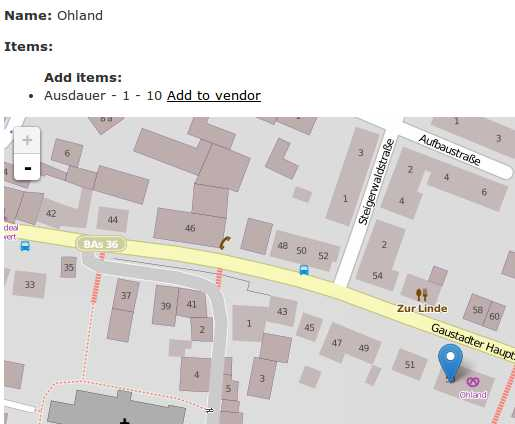
\includegraphics[width=120mm]{images/ch8_item2.png}
\caption{Itempflege - Zuweisen}
\label{img:ch8_item2}
\end{center}
\end{figure}

\begin{figure}[H]
\begin{center}
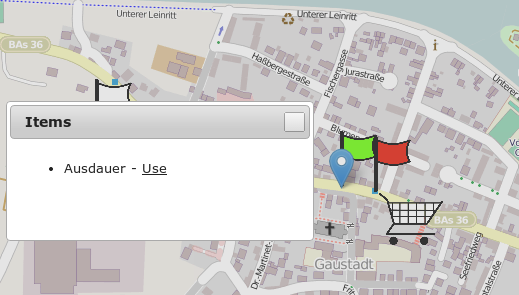
\includegraphics[height=70mm]{images/ch8_item3.png}
\caption{Spielfeld - Itembenutzung}
\label{img:ch8_item3}
\end{center}
\end{figure}

\begin{figure}[H]
\begin{center}
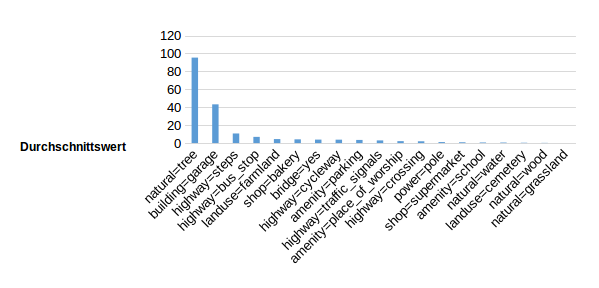
\includegraphics[width=150mm]{images/ch8_valued3.png}
\caption{Bewertung der einzelnen Tags}
\label{img:ch8_valued3}
\end{center}
\end{figure}

\newpage

\section{Quellcode}

Aufgrund des Umfangs und des Entwicklungsvorgehens wurde der Quellcode des Frameworks nicht als optisches Medium beigelegt sondern befindet sich in einem Subversion Repository.
Somit kann das Framework offen von jedem verwendet werden, der ein Interesse daran hat. Soweit nicht anders angegeben steht der Quellcode des Autors unter der GNU GPL v2.
Der Quellcode des Frameworks, Evaluationstools und der Latex Quellcode dieser Arbeit findet sich auf dem Subversion Server von Google Code.
Mit nachfolgender URL kann die entsprechende Version ausgecheckt werden:\\\\
\url{http://geogame-project.googlecode.com/svn/trunk/}\\\\

Die Struktur des Repositorys ist wie folgt:
\begin{itemize}
\item latex - Latex Quellcode dieser Arbeit
\item src - Ruby Quellcode des Frameworks
\item src\_evalTags - Java Quellcode des Evaluationstools
\end{itemize}

\section{Installation}

Für die Ausführung des Frameworks wird Ruby in Version 2.0 und Rails in Version 4.0 benötigt. Letzteres wird automatishc per Bundler installiert.
Darüber hinaus muss sichergestellt werden, dass der Server/Rechner eine aktive Verbindung zum Internet hat, damit die OSM -Daten abgerufen werden können.

Für die Installation des Frameworks ist es ausreichend das Ruby on Rails Projekt per svn auszuchecken:\\\\

\lstset{
   language=Bash
}

\begin{lstlisting}[caption=CLI-Befehl für Code Checkout, label=code:ch8:bash01]
svn checkout http://geogame-project.googlecode.com/svn/trunk/src/
\end{lstlisting}

Danach kann die Anwendung einfach im Projekt-Verzeichnis gestartet werden:\\\\

\begin{lstlisting}[caption=CLI-Befehl für Start des Frameworks, label=code:ch8:bash02]
bundle install;rails s
\end{lstlisting}